\documentclass[aspectratio=169]{beamer}
%\documentclass{beamer}
% changed aspect ratio to 16:9 to match the background image; still works even if this is removed
\setbeamertemplate{navigation symbols}{}
\setbeamercolor{frametitle}{fg=red}
\setbeamercolor{title}{fg=white}
\setbeamercolor{author}{fg=white}
\setbeamercolor{date}{fg=white}
\setbeamerfont{frametitle}{family=\rmfamily,shape=\itshape,size=\huge} 
\setbeamerfont{title}{family=\rmfamily,shape=\itshape,size=\huge} 
\usetheme{boxes}
\setbeamertemplate{footline}[frame number]
\setbeamertemplate{itemize/enumerate body begin}{\small}
\setbeamertemplate{itemize/enumerate subbody begin}{\footnotesize}
%
%Global Background must be put in preamble
%-rescale the 16:9 image to slide size choice
\usebackgroundtemplate{
\includegraphics[width=\paperwidth,height=\paperheight]{bnl_interior}}
%
\title{Cosmology with the Dark Energy Survey}
\author{Erin Sheldon}
\date{July 25, 2018}
%
\begin{document}
{\usebackgroundtemplate{
\includegraphics[width=\paperwidth,height=\paperheight]{bnl_title}}
\maketitle
}


%
\frame
{

    \frametitle{The Dark Energy Survey}

    %\setbeamerfont*{itemize/enumerate body}{size=\large}

    \begin{columns}
        \begin{column}{0.5\textwidth}
            \centering
                \includegraphics[height=0.8\textheight]{ctio_blanco_crew_2013Oct-30-small-balance.jpg}
                \newline
                {\tiny Image Brian Nord}
        \end{column}

        \begin{column}{0.5\textwidth}
            \begin{itemize}

                \item DES is a 5 year optical imaging survey covering 5000
                    square degrees of the southern sky in 5 filters.

                \item New camera DECam, built at FNAL, placed on existing 4
                    meter telescope at CTIO in Chile.

                \item The goal is to study dark energy using four primary probes:  
                    \begin{itemize}
                        \item Weak Gravitational Lensing
                        \item Clusters of Galaxies
                        \item Galaxy clustering
                        \item Supernovae
                    \end{itemize}

            \end{itemize}

        \end{column}

    \end{columns}


}

\frame
{

    \frametitle{Current Status}

    %\setbeamerfont*{itemize/enumerate body}{size=\large}

    \begin{columns}
        \begin{column}{0.5\textwidth}
            \begin{itemize}

                \item Finished taking 5th year of data.

                \item Cosmology results released for year 1 data.

                \item Working on year 3 cosmology results now.

                \item The data is beautiful!

            \end{itemize}

        \end{column}
        \begin{column}{0.5\textwidth}
            \centering
                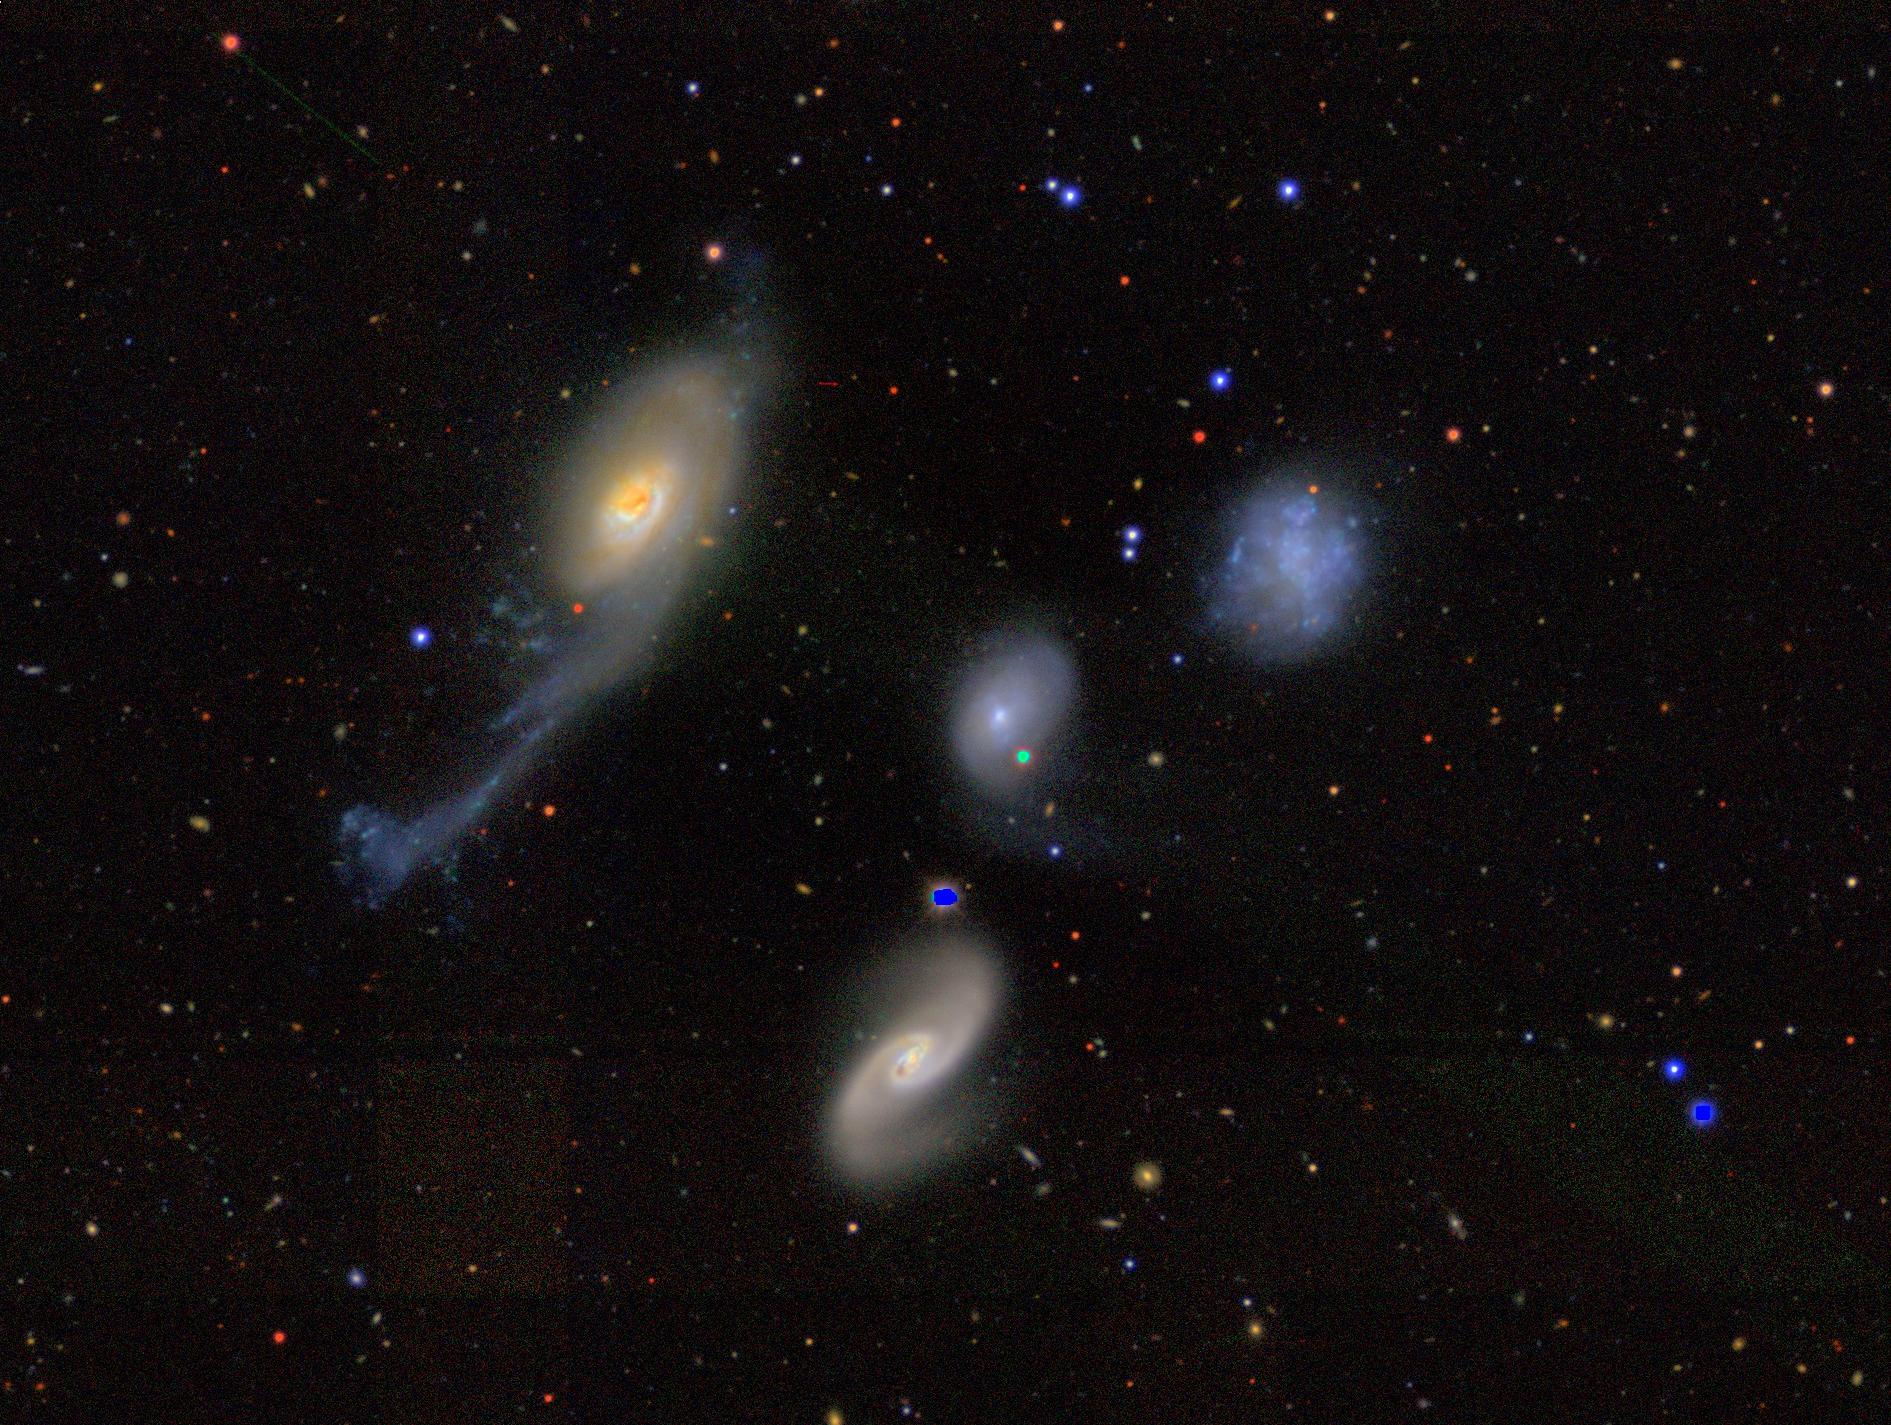
\includegraphics[width=\linewidth]{DES0022-4831-four.jpg}
                \newline
                {\tiny DES/Erin Sheldon}
        \end{column}

    \end{columns}


}



{
    \usebackgroundtemplate{%
        \colorbox{black}{ \parbox[c][\paperheight][c]{\paperwidth}{\centering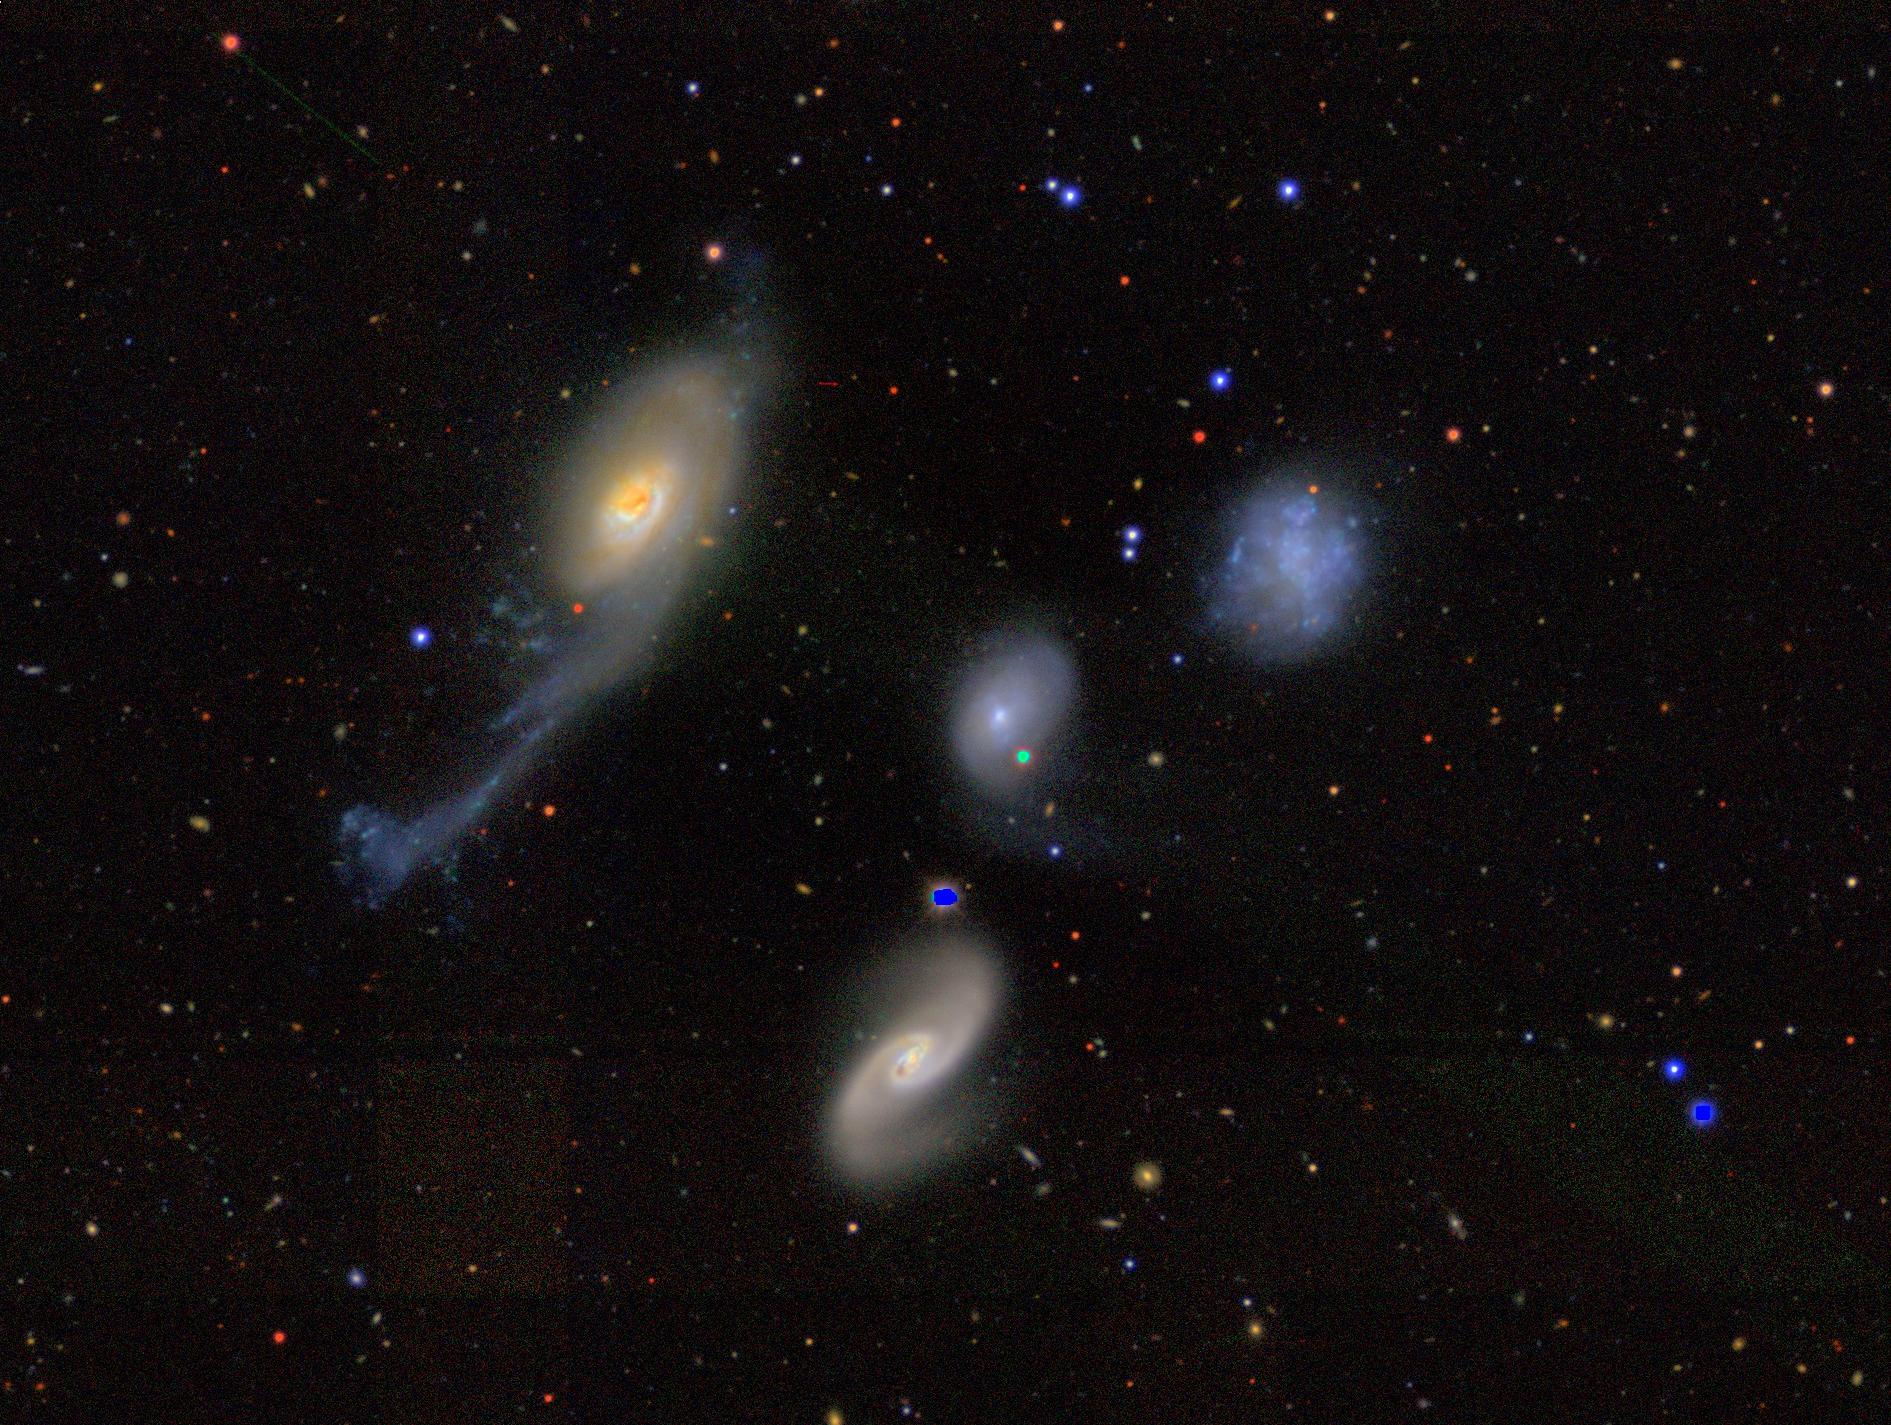
\includegraphics[height=\paperheight]{DES0022-4831-four.jpg}} }
        %\colorbox{black}{ \vbox to \paperheight{\vfil\hbox to \paperwidth{\hfil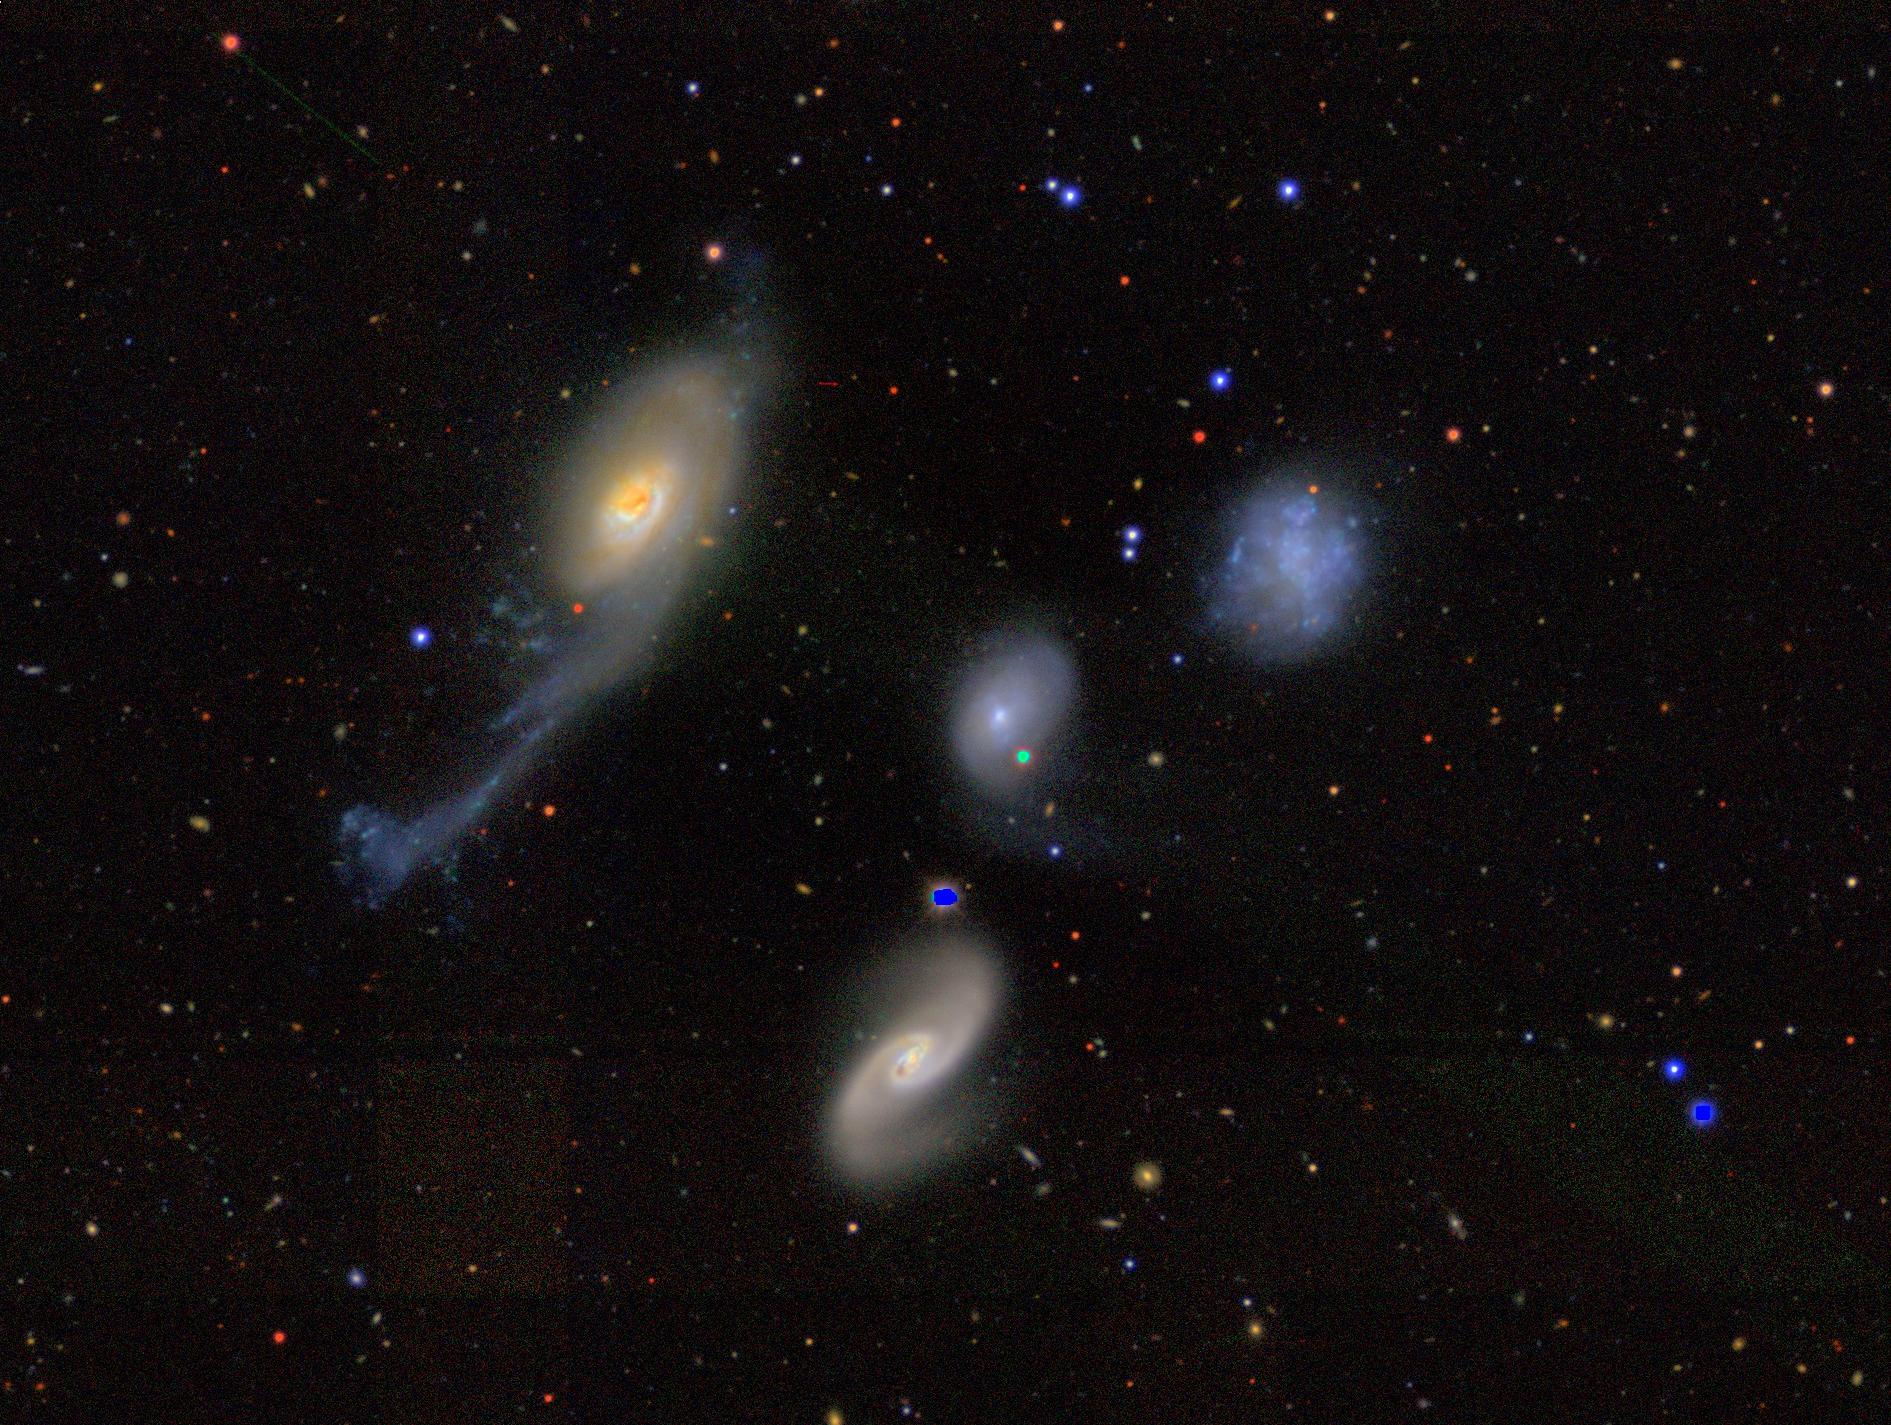
\includegraphics[height=\paperheight]{DES0022-4831-four.jpg}\hfil}\vfil} }
    }
\frame
{
}
}


{
    \usebackgroundtemplate{%
        \includegraphics[height=\paperheight]{DES-2013-01-medres.jpg}}
\frame
{
}
}

{
    \usebackgroundtemplate{%
        \colorbox{black}{ \parbox[c][\paperheight][c]{\paperwidth}{\centering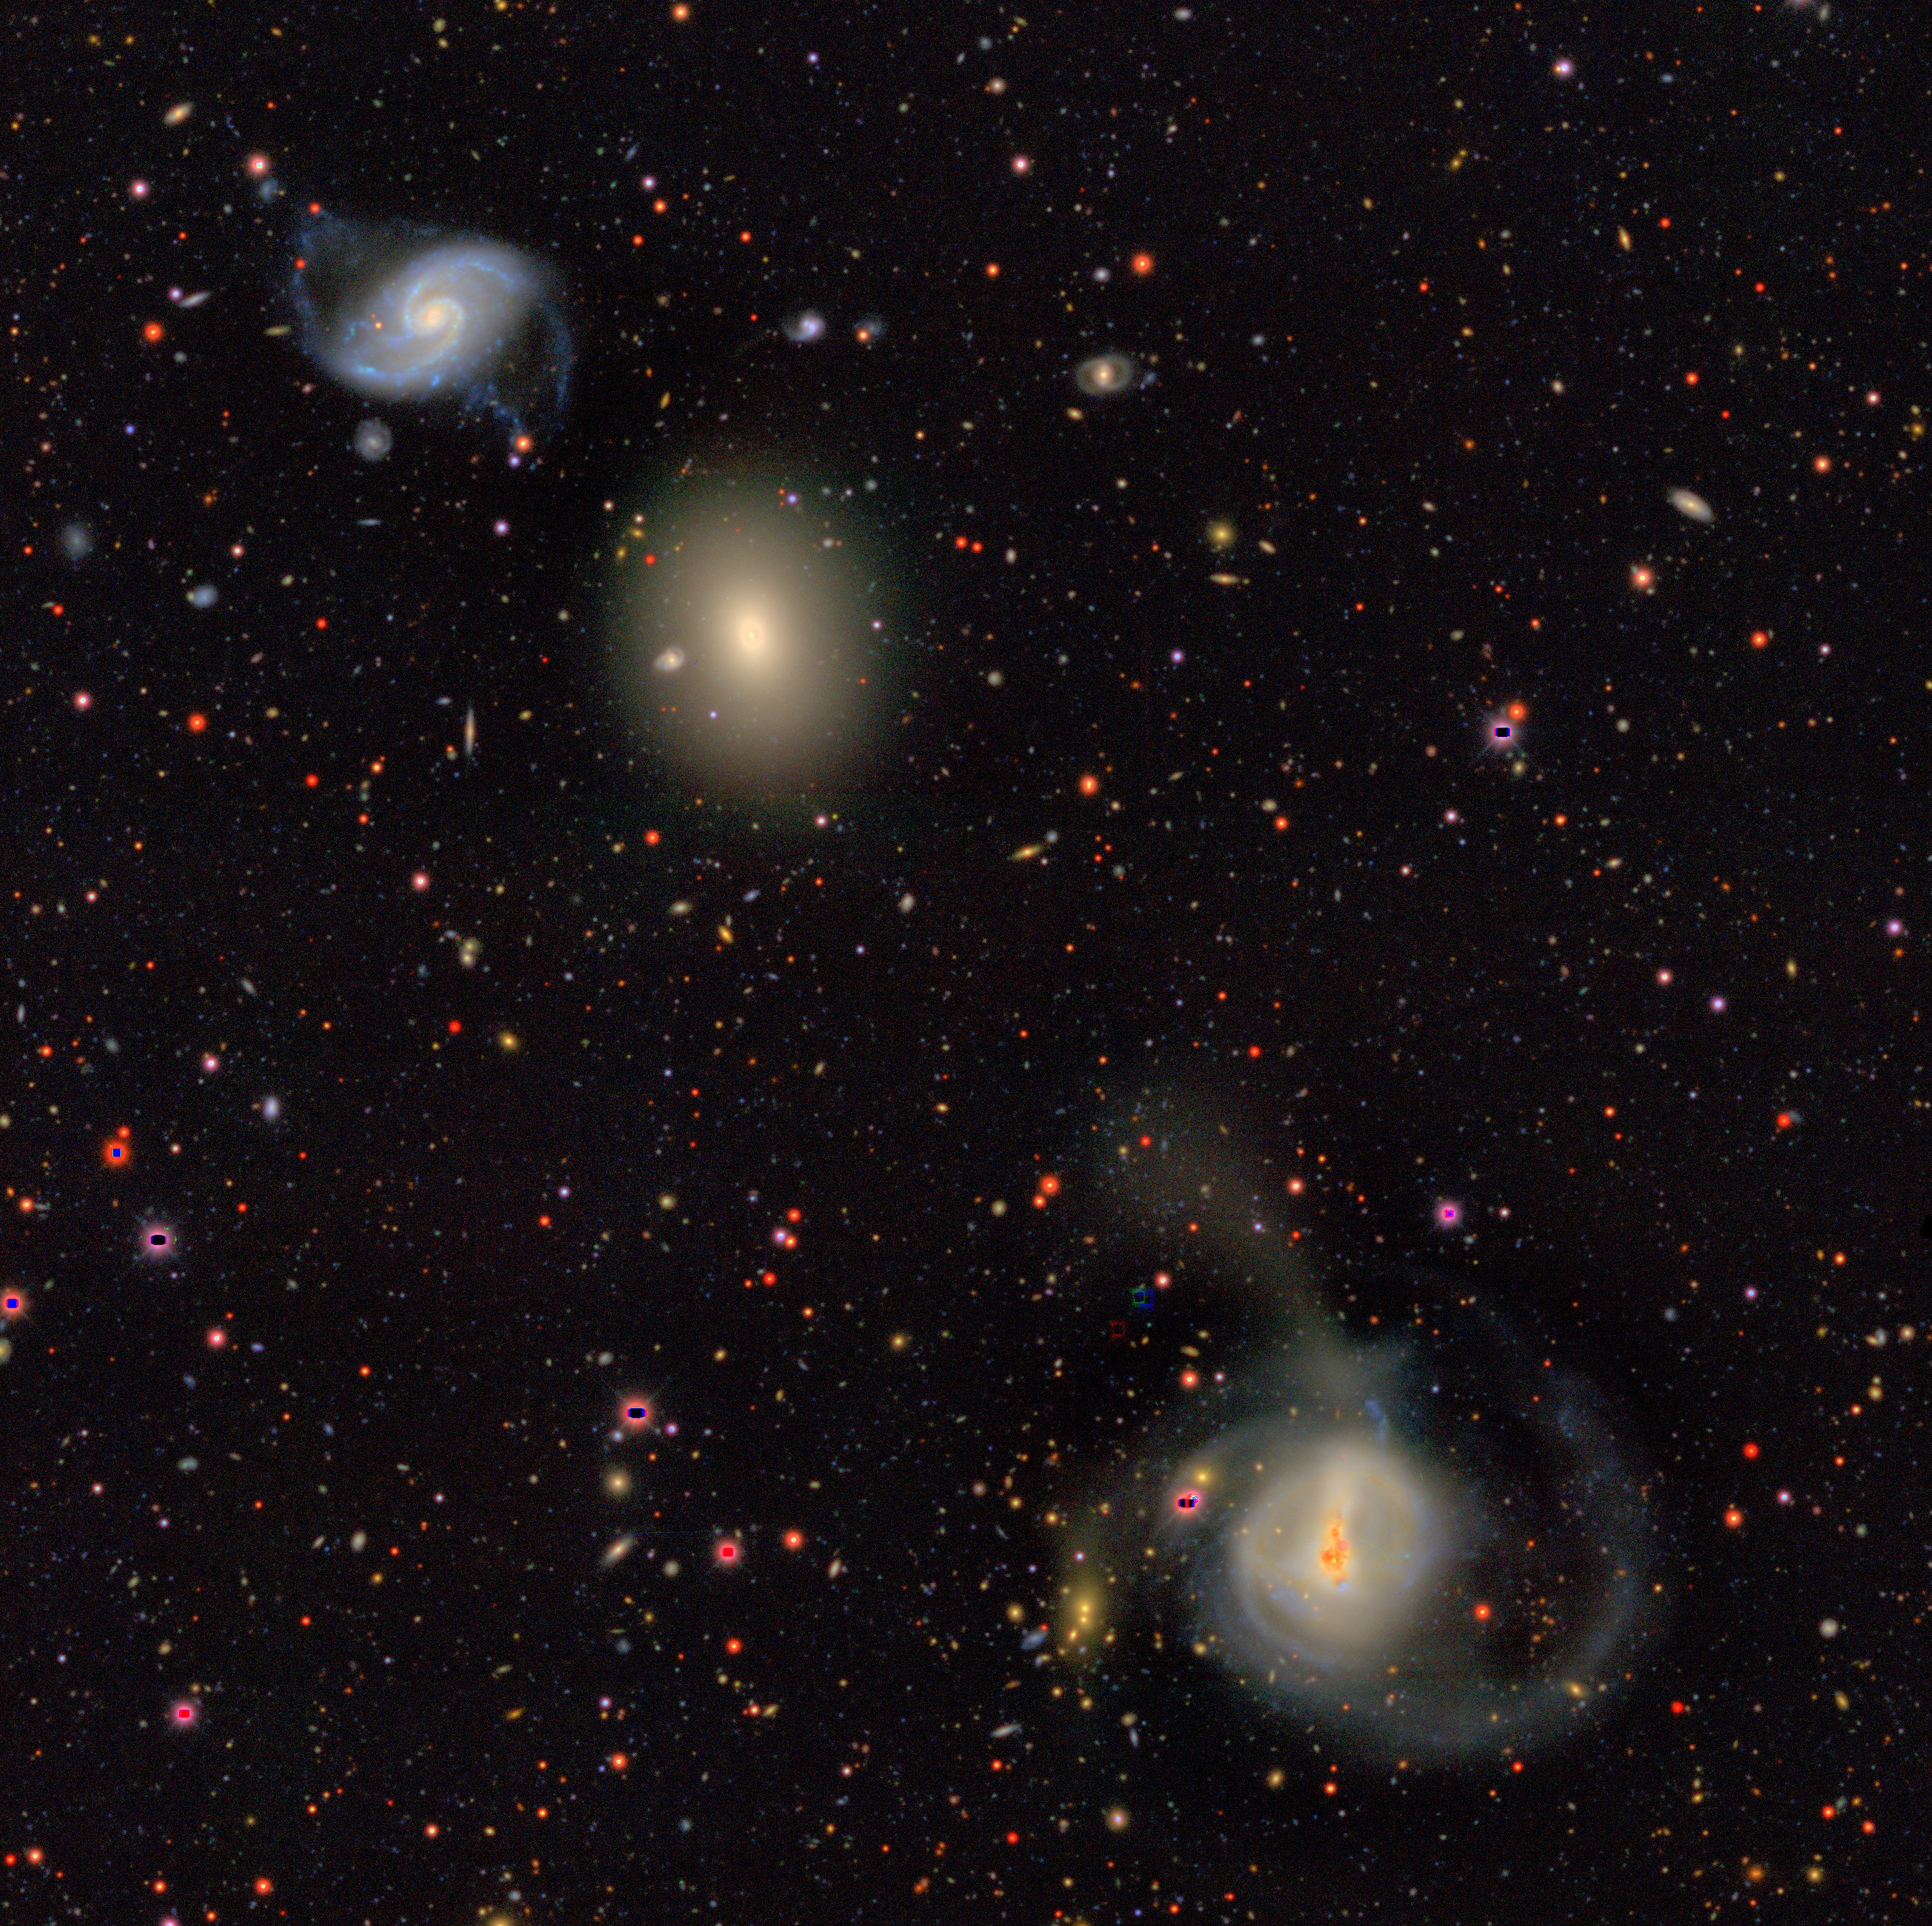
\includegraphics[height=\paperheight]{DES0428-4748_gri_sv_mask_streaks_color_trim.jpg}} }
    }
\frame
{
}
}

{
    \usebackgroundtemplate{%
        \colorbox{black}{ \parbox[c][\paperheight][c]{\paperwidth}{\centering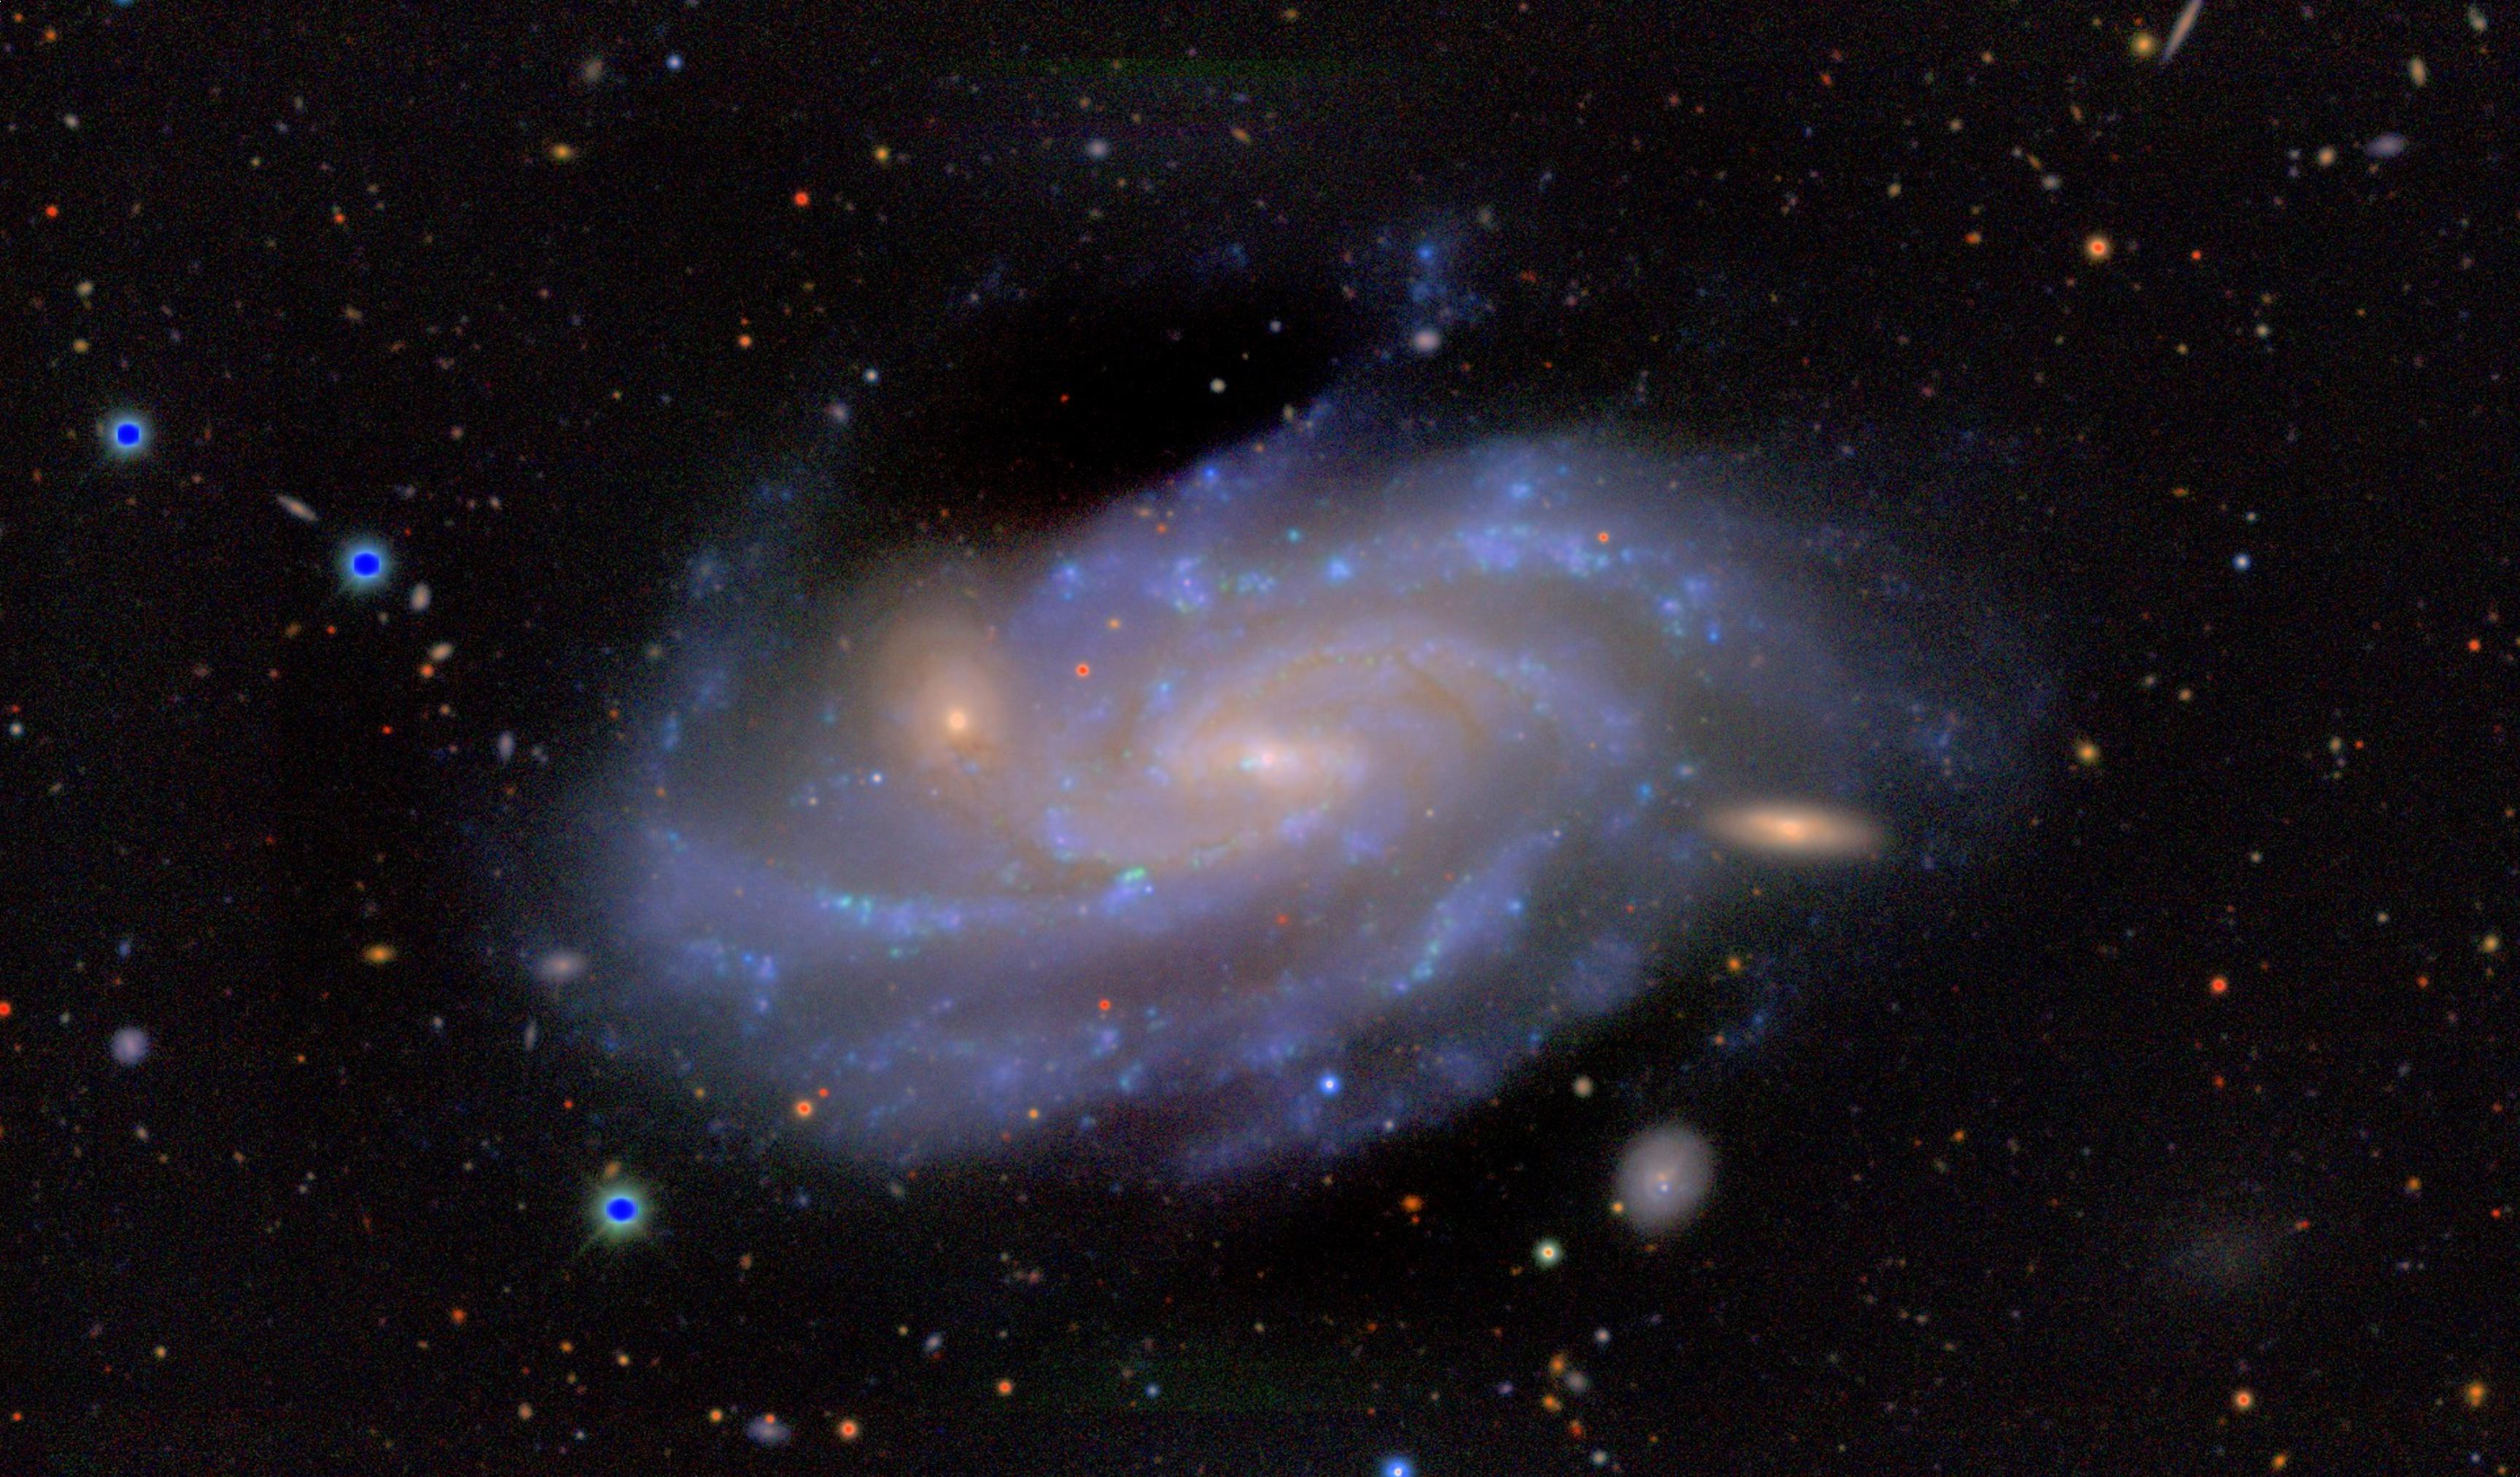
\includegraphics[height=\paperheight]{DES0130-2249-nearby-projection.jpg}} }
    }
\frame
{
}
}

{
    \usebackgroundtemplate{%
        \colorbox{black}{ \parbox[c][\paperheight][c]{\paperwidth}{\centering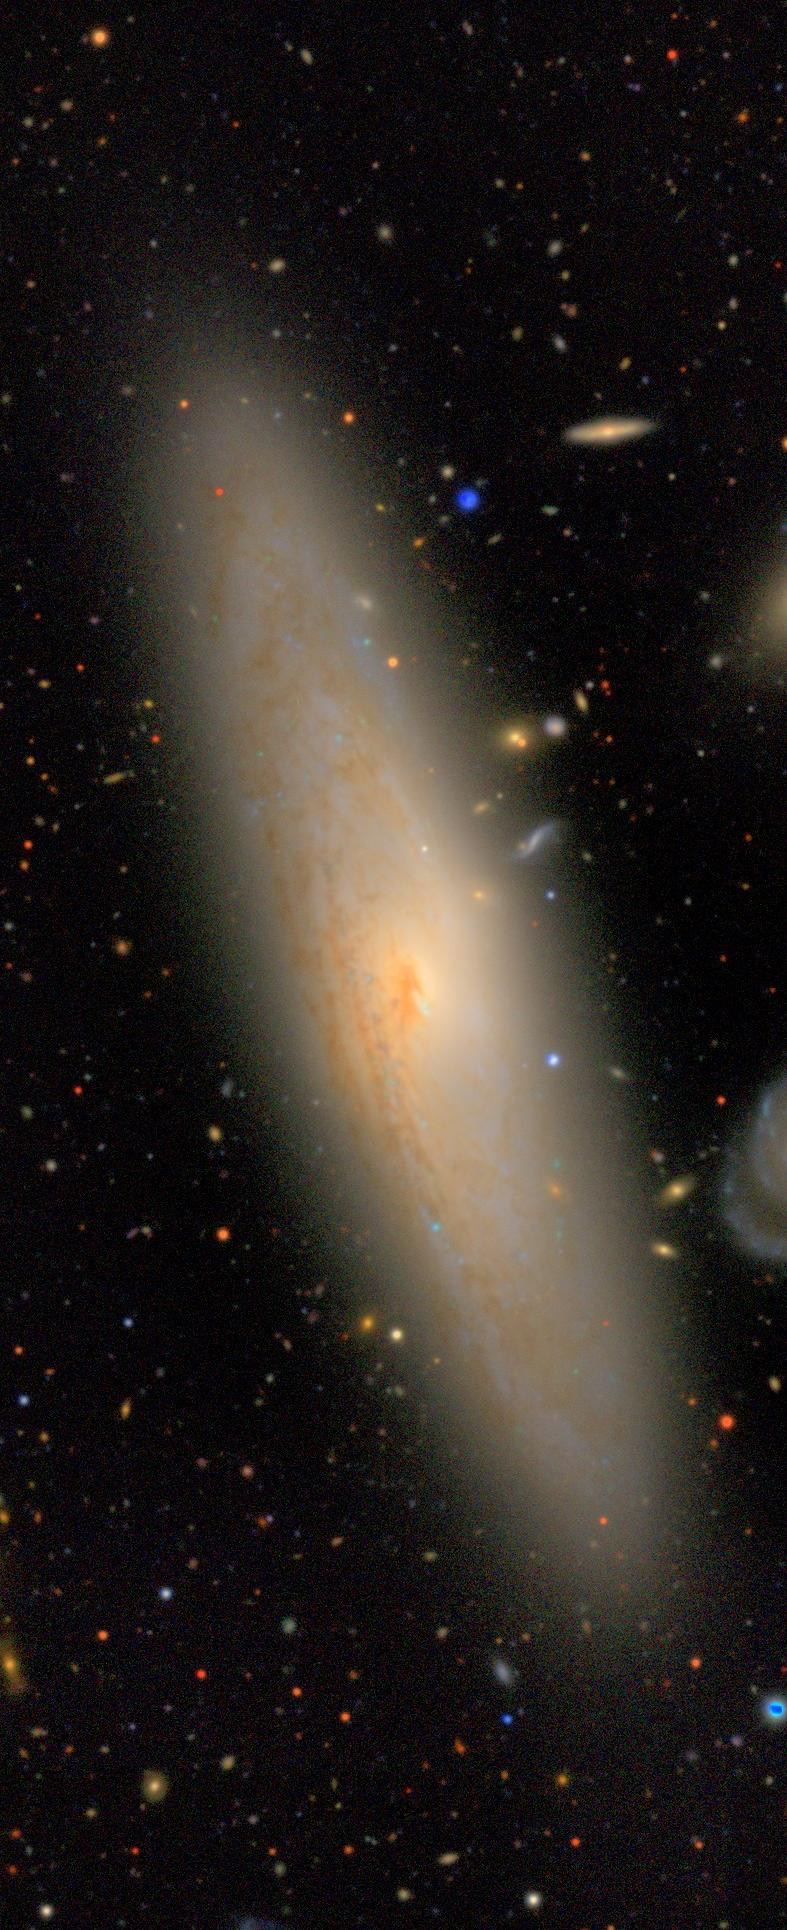
\includegraphics[width=0.7\paperheight,angle=90]{DES0406-5414-huge.jpg}} }
    }
\frame
{
}
}

{
    \usebackgroundtemplate{%
        \colorbox{black}{ \parbox[c][\paperheight][c]{\paperwidth}{\centering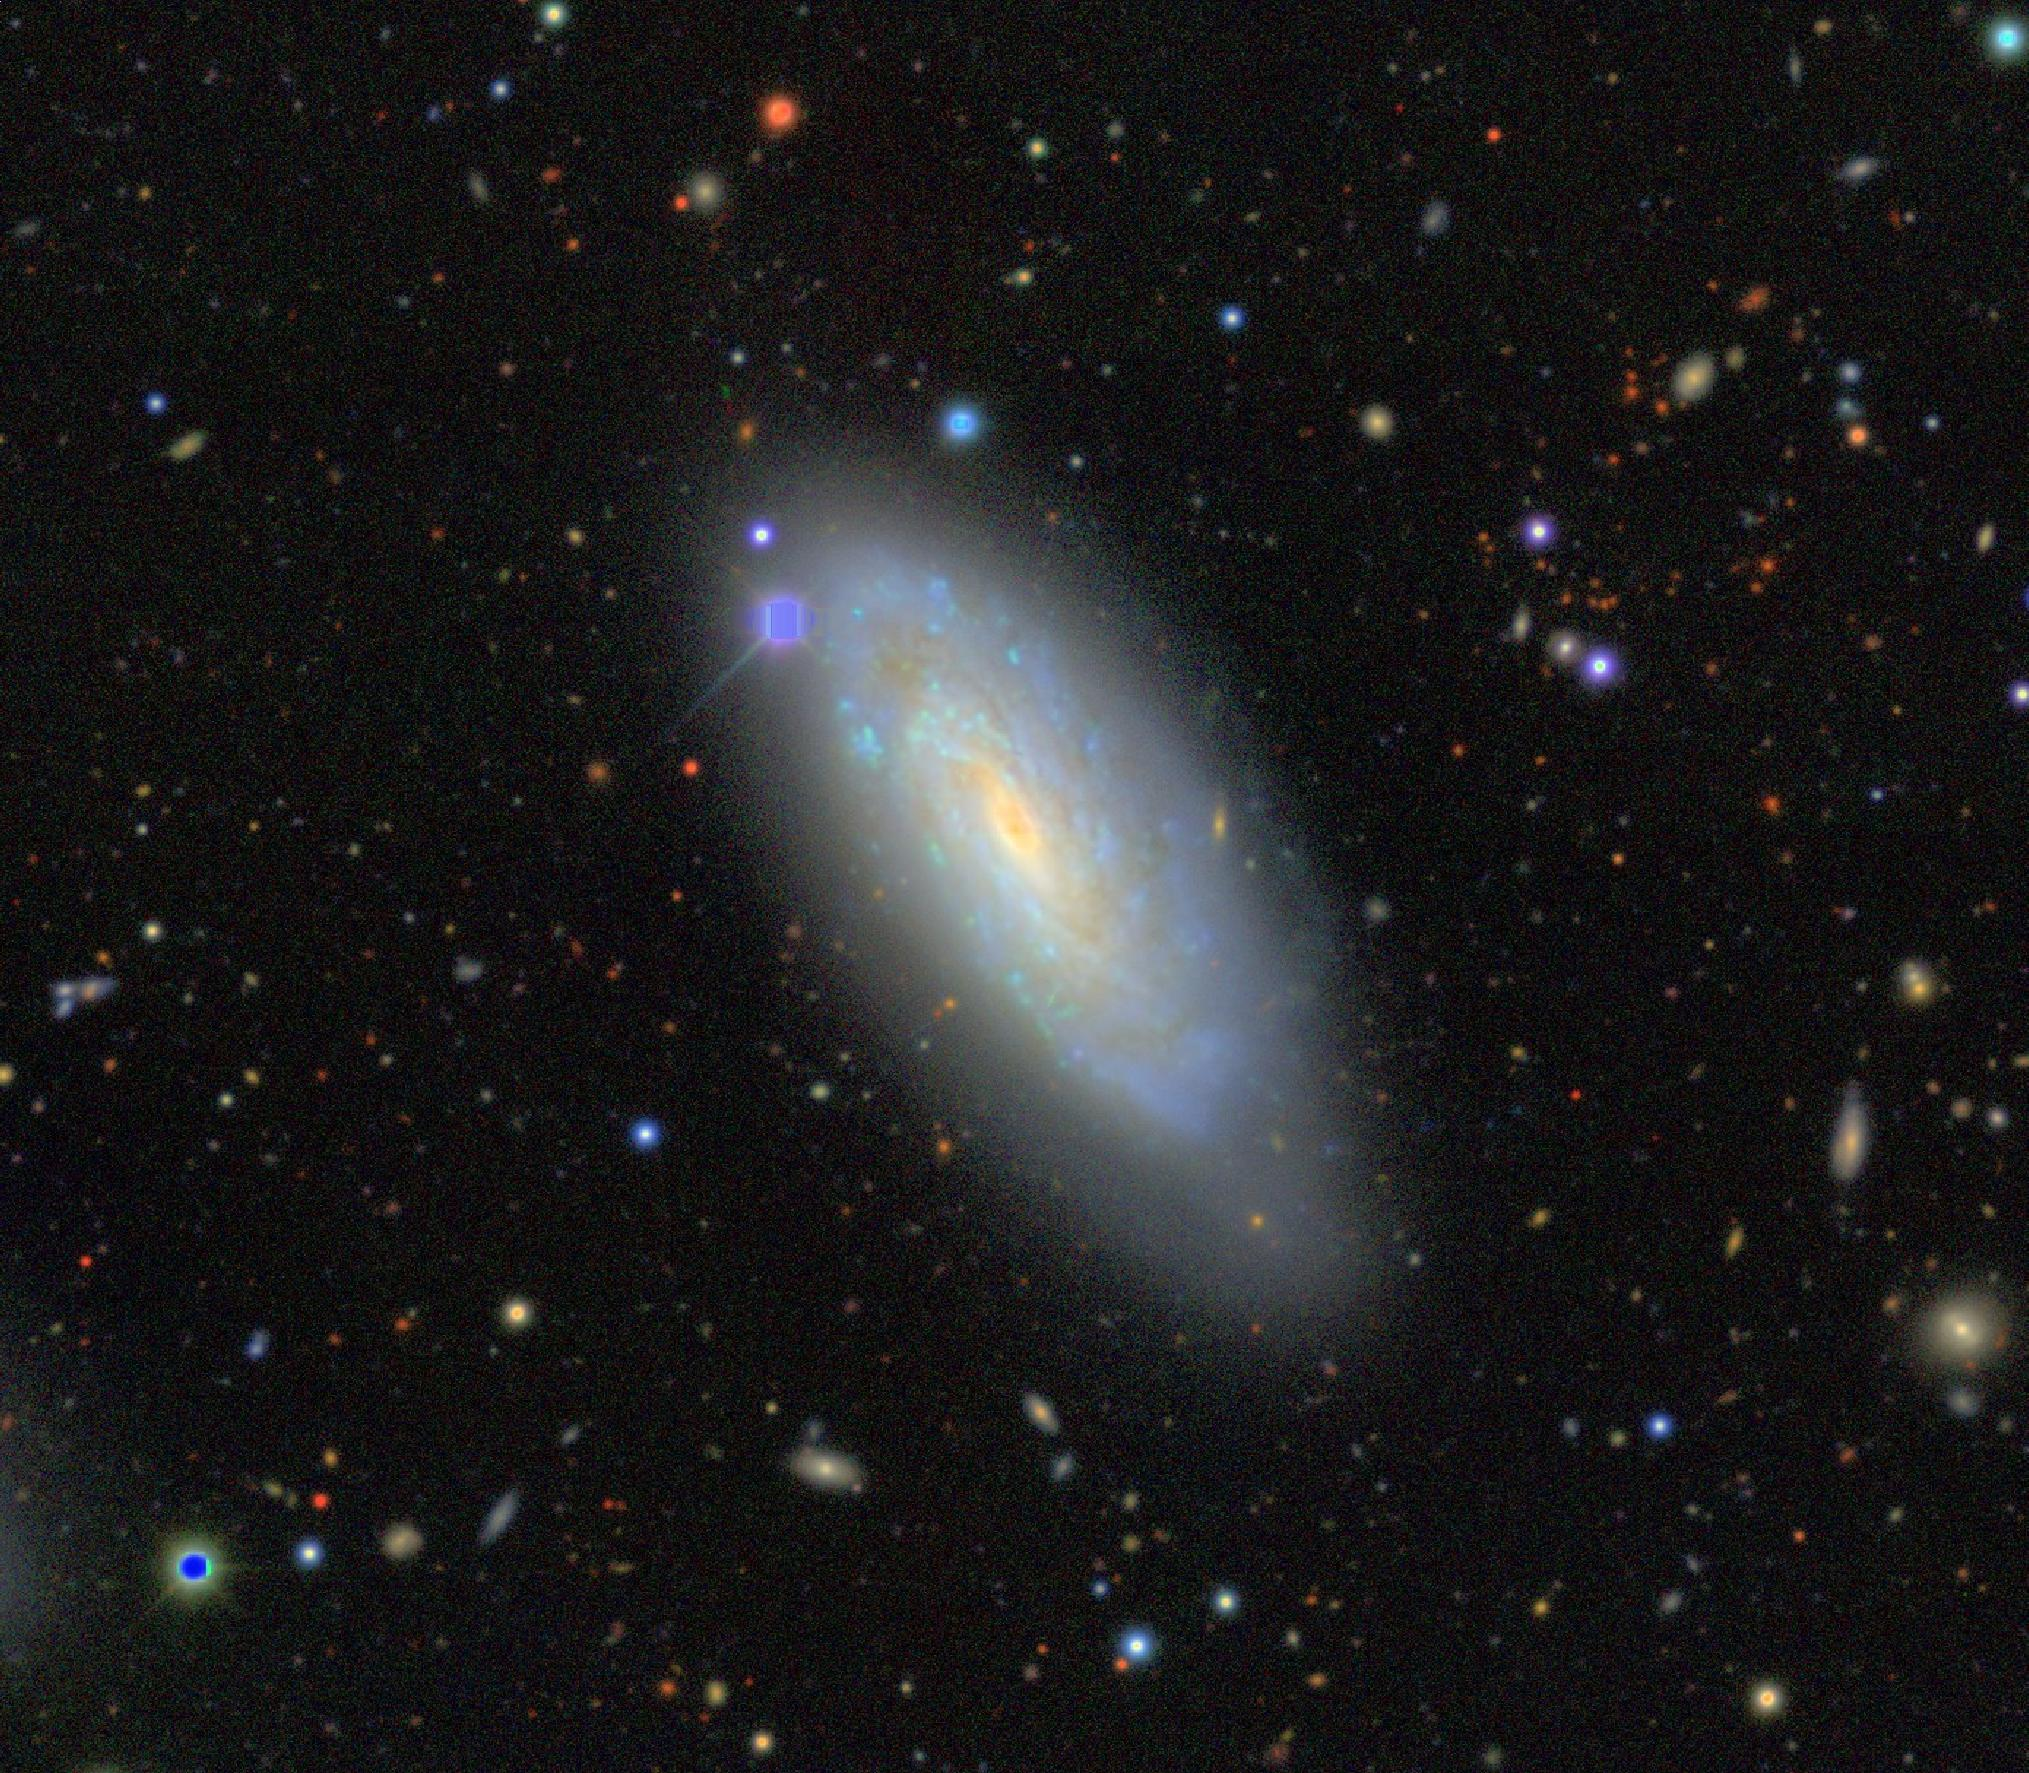
\includegraphics[height=\paperheight]{DES2320-4206-spiral.jpg}} }
    }
\frame
{
}
}








\end{document}
